\documentclass[tikz]{standalone}
\begin{document}
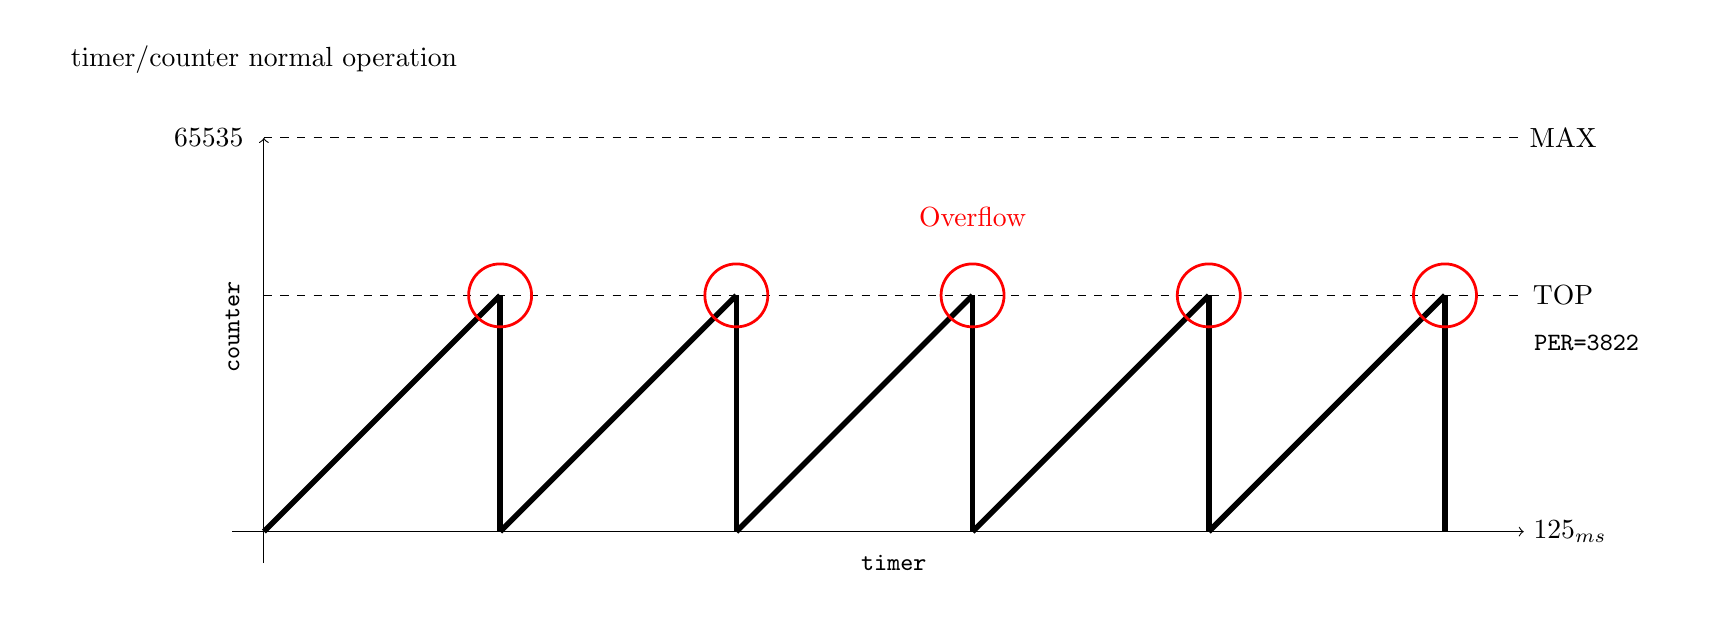
\begin{tikzpicture}[scale=2]
\useasboundingbox (-1.5,-0.5) rectangle (9,3.2);
\node at (0,3) {timer/counter normal operation};

\draw[->] (-0.2, 0.0) -- (8,0.0) node[right] {$125_{ms}$};
\draw[->] ( 0.0,-0.2) -- (0,2.5);

\node[font=\small\ttfamily] at (4.0,-0.2) {timer};
\node[font=\small\ttfamily, rotate=90] at (-0.2,1.3) {counter};

\draw[dashed, thin, black] (0,2.5) -- (8,2.5) node[xshift=5mm] {MAX} node[pos=0, xshift=-7mm] {65535};
\draw[dashed, thin, black] (0,1.5) -- (8,1.5) node[xshift=5mm] {TOP};
\draw[font=\small\ttfamily] (8.4,1.2) node {PER=3822};

\foreach \x in {0.0,1.5,...,6} {
	\draw[line width=2pt] (\x+0.0,0.0) -- (\x+1.5,1.5);
	\draw[line width=2pt] (\x+1.5,1.5) -- (\x+1.5,0.0);
	\draw[draw=red, line width=1pt] (\x+1.5,1.5) circle (0.2cm);
}

\node[text=red] at (4.5,2) {Overflow};
\end{tikzpicture}
\end{document}